%%=============================================================================
%% LaTeX sjabloon voor bachelorproef, HoGent Bedrijf en Organisatie
%% Opleiding Toegepaste Informatica
%%=============================================================================

\documentclass[fleqn,a4paper,12pt]{book}

%%=============================================================================
%% LaTeX sjabloon voor de bachelorproef, HoGent Bedrijf en Organisatie
%% Opleiding toegepaste informatica
%%
%% Structuur en algemene vormgeving. Meestal hoef je hier niets te wijzigen.
%%
%% Vormgeving gebaseerd op "The Legrand Orange Book", version 2.0 (9/2/15)
%% door Mathias Legrand (legrand.mathias@gmail.com) met aanpassingen door
%% Vel (vel@latextemplates.com). Het oorspronkelijke template is te vinden op
%% http://www.LaTeXTemplates.com
%%
%% Aanpassingen voor HoGent toegepaste informatica: 
%%   Bert Van Vreckem <bert.vanvreckem@hogent.be>
%% Licentie: 
%%   CC BY-NC-SA 3.0 (http://creativecommons.org/licenses/by-nc-sa/3.0/)
%%=============================================================================

%%-----------------------------------------------------------------------------
%% Packages
%%-----------------------------------------------------------------------------

\usepackage[top=3cm,bottom=3cm,left=3cm,right=3cm,headsep=10pt,a4paper]{geometry} % Page margins
\usepackage[utf8]{inputenc}  % Accenten gebruiken in tekst (vb. é ipv \'e)
\usepackage{amsfonts}        % AMS math packages: extra wiskundige
\usepackage{amsmath}         %   symbolen (o.a. getallen-
\usepackage{amssymb}         %   verzamelingen N, R, Z, Q, etc.)
\usepackage[english,dutch]{babel}    % Taalinstellingen: woordsplitsingen,
                             %  commando's voor speciale karakters
                             %  ("dutch" voor NL)
\usepackage{iflang}
\usepackage{eurosym}         % Euro-symbool €
\usepackage{geometry}
\usepackage{graphicx}        % Invoegen van tekeningen
\graphicspath{{img/}}       % Specifies the directory where pictures are stored
\usepackage{tikz}            % Required for drawing custom shapes
\usepackage[pdftex,bookmarks=true]{hyperref}
                             % PDF krijgt klikbare links & verwijzingen,
                             %  inhoudstafel
\usepackage{enumitem}        % Customize lists
\setlist{nolistsep}         % Reduce spacing between list items
\usepackage{listings}        % Broncode mooi opmaken
\lstset{
	basicstyle=\ttfamily,
	frame=single
}
\usepackage{color}
\usepackage{multirow}        % Tekst over verschillende cellen in tabellen
\usepackage{rotating}        % Tabellen en figuren roteren

\usepackage{booktabs}        % Required for nicer horizontal rules in tables

\usepackage{xcolor}          % Required for specifying colors by name
\definecolor{maincolor}{RGB}{0,147,208} % Define the main color used for 
                             % highlighting throughout the book
                             % 0, 147, 208 = officiële kleur HoGent FBO

% Paragraph style: no indent, add space between paragraphs
\setlength{\parindent}{0em}
\setlength{\parskip}{1em}

\usepackage{etoolbox}
\usepackage{titling} % Macros for title, author, etc
\usepackage{lipsum}          % Voor vultekst (lorem ipsum)

%----------------------------------------------------------------------------------------
%	FONTS
%----------------------------------------------------------------------------------------

\usepackage{avant} % Use the Avantgarde font for headings
%\usepackage{times} % Use the Times font for headings
\usepackage{mathptmx} % Use the Adobe Times Roman as the default text font together with math symbols from the Sym­bol, Chancery and Com­puter Modern fonts

\usepackage{microtype} % Slightly tweak font spacing for aesthetics
\usepackage[utf8]{inputenc} % Required for including letters with accents
\usepackage[T1]{fontenc} % Use 8-bit encoding that has 256 glyphs

%------------------------------------------------------------------------------
%	TITLE PAGE
%------------------------------------------------------------------------------

\newcommand{\inserttitlepage}{%
\begin{titlepage}
  \newgeometry{top=2cm,bottom=1.5cm,left=1.5cm,right=1.5cm}
  \begin{center}

    \begingroup
    \rmfamily
    
\includegraphics[width=2.5cm]{img/HG-beeldmerk-woordmerk}\\[.5cm]
    Faculteit Bedrijf en Organisatie\\[3cm]
    \titel
    \vfill
    \student\\[3.5cm]
    Scriptie voorgedragen tot het bekomen van de graad van\\professionele bachelor in de toegepaste informatica\\[2cm]
    Promotor:\\
    \promotor\\
    \ifdefempty{\copromotor}{\vspace{2.5cm}}{Co-promotor:\\\copromotor\\[2.5cm]}
    Instelling: \instelling\\[.5cm]
    Academiejaar: \academiejaar\\[.5cm]
    \ifcase \examenperiode \or Eerste \or Tweede \else Derde \fi examenperiode
    \endgroup

  \end{center}
  \restoregeometry
\end{titlepage}
  \emptypage
\begin{titlepage}
  \newgeometry{top=5.35cm,bottom=1.5cm,left=1.5cm,right=1.5cm}
  \begin{center}

    \begingroup
    \rmfamily
    \IfLanguageName{dutch}{Faculteit Bedrijf en Organisatie}{Faculty of Business and Information Management}\\[3cm]
    \titel
    \vfill
    \student\\[3.5cm]
    \IfLanguageName{dutch}{Scriptie voorgedragen tot het bekomen van de graad van\\professionele bachelor in de toegepaste informatica}{Thesis submitted in partial fulfilment of the requirements for the degree of\\professional bachelor of applied computer science}\\[2cm]
    Promotor:\\
    \promotor\\
    \ifdefempty{\copromotor}{\vspace{2.5cm}}{Co-promotor:\\\copromotor\\[2.5cm]}
    \IfLanguageName{dutch}{Instelling}{Institution}: \instelling\\[.5cm]
    \IfLanguageName{dutch}{Academiejaar}{Academic year}: \academiejaar\\[.5cm]
    \IfLanguageName{dutch}{%
    \ifcase \examenperiode \or Eerste \or Tweede \else Derde \fi examenperiode}{%
    \ifcase \examenperiode \or First \or Second \else Third \fi examination period}
    \endgroup

  \end{center}
  \restoregeometry
\end{titlepage}
}

%----------------------------------------------------------------------------------------
%	BIBLIOGRAPHY AND INDEX
%----------------------------------------------------------------------------------------

\usepackage[style=apa,backend=biber]{biblatex}
\usepackage{csquotes}
\DeclareLanguageMapping{dutch}{dutch-apa}
\addbibresource{bachproef-tin.bib} % BibTeX bibliography file
\addbibresource{../voorstel/voorstel.bib}
\defbibheading{bibempty}{}

\usepackage{calc} % For simpler calculation - used for spacing the index letter headings correctly
\usepackage{makeidx} % Required to make an index
\makeindex % Tells LaTeX to create the files required for indexing

%----------------------------------------------------------------------------------------
%	MAIN TABLE OF CONTENTS
%----------------------------------------------------------------------------------------

\usepackage{titletoc} % Required for manipulating the table of contents

\contentsmargin{0cm} % Removes the default margin

% Part text styling
\titlecontents{part}[0cm]
{\addvspace{20pt}\centering\large\bfseries}
{}
{}
{}

% Chapter text styling
\titlecontents{chapter}[1.25cm] % Indentation
{\addvspace{12pt}\large\sffamily\bfseries} % Spacing and font options for chapters
{\color{maincolor!60}\contentslabel[\Large\thecontentslabel]{1.25cm}\color{maincolor}} % Chapter number
{\color{maincolor}}
{\color{maincolor!60}\normalsize\;\titlerule*[.5pc]{.}\;\thecontentspage} % Page number

% Section text styling
\titlecontents{section}[1.25cm] % Indentation
{\addvspace{3pt}\sffamily\bfseries} % Spacing and font options for sections
{\contentslabel[\thecontentslabel]{1.25cm}} % Section number
{}
{\hfill\color{black}\thecontentspage} % Page number
[]

% Subsection text styling
\titlecontents{subsection}[1.25cm] % Indentation
{\addvspace{1pt}\sffamily\small} % Spacing and font options for subsections
{\contentslabel[\thecontentslabel]{1.25cm}} % Subsection number
{}
{\ \titlerule*[.5pc]{.}\;\thecontentspage} % Page number
[]

% List of figures
\titlecontents{figure}[0em]
{\addvspace{-5pt}\sffamily}
{\thecontentslabel\hspace*{1em}}
{}
{\ \titlerule*[.5pc]{.}\;\thecontentspage}
[]

% List of tables
\titlecontents{table}[0em]
{\addvspace{-5pt}\sffamily}
{\thecontentslabel\hspace*{1em}}
{}
{\ \titlerule*[.5pc]{.}\;\thecontentspage}
[]

%----------------------------------------------------------------------------------------
%	MINI TABLE OF CONTENTS IN PART HEADS
%----------------------------------------------------------------------------------------

% Chapter text styling
\titlecontents{lchapter}[0em] % Indenting
{\addvspace{15pt}\large\sffamily\bfseries} % Spacing and font options for chapters
{\color{maincolor}\contentslabel[\Large\thecontentslabel]{1.25cm}\color{maincolor}} % Chapter number
{}
{\color{maincolor}\normalsize\sffamily\bfseries\;\titlerule*[.5pc]{.}\;\thecontentspage} % Page number

% Section text styling
\titlecontents{lsection}[0em] % Indenting
{\sffamily\small} % Spacing and font options for sections
{\contentslabel[\thecontentslabel]{1.25cm}} % Section number
{}
{}

% Subsection text styling
\titlecontents{lsubsection}[.5em] % Indentation
{\normalfont\footnotesize\sffamily} % Font settings
{}
{}
{}

%----------------------------------------------------------------------------------------
%	PAGE HEADERS
%----------------------------------------------------------------------------------------

\usepackage{fancyhdr} % Required for header and footer configuration

\pagestyle{fancy}
\renewcommand{\chaptermark}[1]{\markboth{\sffamily\normalsize\bfseries\chaptername\ \thechapter.\ #1}{}} % Chapter text font settings
\renewcommand{\sectionmark}[1]{\markright{\sffamily\normalsize\thesection\hspace{5pt}#1}{}} % Section text font settings
\fancyhf{} \fancyhead[LE,RO]{\sffamily\normalsize\thepage} % Font setting for the page number in the header
\fancyhead[LO]{\rightmark} % Print the nearest section name on the left side of odd pages
\fancyhead[RE]{\leftmark} % Print the current chapter name on the right side of even pages
\renewcommand{\headrulewidth}{0.5pt} % Width of the rule under the header
\addtolength{\headheight}{2.5pt} % Increase the spacing around the header slightly
\renewcommand{\footrulewidth}{0pt} % Removes the rule in the footer
\fancypagestyle{plain}{\fancyhead{}\renewcommand{\headrulewidth}{0pt}} % Style for when a plain pagestyle is specified

% Removes the header from odd empty pages at the end of chapters
\makeatletter
\renewcommand{\cleardoublepage}{
\clearpage\ifodd\c@page\else
\hbox{}
\vspace*{\fill}
\thispagestyle{empty}
\newpage
\fi}

%----------------------------------------------------------------------------------------
%	THEOREM STYLES
%----------------------------------------------------------------------------------------

\usepackage{amsmath,amsfonts,amssymb,amsthm} % For math equations, theorems, symbols, etc

\newcommand{\intoo}[2]{\mathopen{]}#1\,;#2\mathclose{[}}
\newcommand{\ud}{\mathop{\mathrm{{}d}}\mathopen{}}
\newcommand{\intff}[2]{\mathopen{[}#1\,;#2\mathclose{]}}
\newtheorem{notation}{Notation}[chapter]

% Boxed/framed environments
\newtheoremstyle{maincolornumbox}% % Theorem style name
{0pt}% Space above
{0pt}% Space below
{\normalfont}% % Body font
{}% Indent amount
{\small\bf\sffamily\color{maincolor}}% % Theorem head font
{\;}% Punctuation after theorem head
{0.25em}% Space after theorem head
{\small\sffamily\color{maincolor}\thmname{#1}\nobreakspace\thmnumber{\@ifnotempty{#1}{}\@upn{#2}}% Theorem text (e.g. Theorem 2.1)
\thmnote{\nobreakspace\the\thm@notefont\sffamily\bfseries\color{black}---\nobreakspace#3.}} % Optional theorem note
\renewcommand{\qedsymbol}{$\blacksquare$}% Optional qed square

\newtheoremstyle{blacknumex}% Theorem style name
{5pt}% Space above
{5pt}% Space below
{\normalfont}% Body font
{} % Indent amount
{\small\bf\sffamily}% Theorem head font
{\;}% Punctuation after theorem head
{0.25em}% Space after theorem head
{\small\sffamily{\tiny\ensuremath{\blacksquare}}\nobreakspace\thmname{#1}\nobreakspace\thmnumber{\@ifnotempty{#1}{}\@upn{#2}}% Theorem text (e.g. Theorem 2.1)
\thmnote{\nobreakspace\the\thm@notefont\sffamily\bfseries---\nobreakspace#3.}}% Optional theorem note

\newtheoremstyle{blacknumbox} % Theorem style name
{0pt}% Space above
{0pt}% Space below
{\normalfont}% Body font
{}% Indent amount
{\small\bf\sffamily}% Theorem head font
{\;}% Punctuation after theorem head
{0.25em}% Space after theorem head
{\small\sffamily\thmname{#1}\nobreakspace\thmnumber{\@ifnotempty{#1}{}\@upn{#2}}% Theorem text (e.g. Theorem 2.1)
\thmnote{\nobreakspace\the\thm@notefont\sffamily\bfseries---\nobreakspace#3.}}% Optional theorem note

% Non-boxed/non-framed environments
\newtheoremstyle{maincolornum}% % Theorem style name
{5pt}% Space above
{5pt}% Space below
{\normalfont}% % Body font
{}% Indent amount
{\small\bf\sffamily\color{maincolor}}% % Theorem head font
{\;}% Punctuation after theorem head
{0.25em}% Space after theorem head
{\small\sffamily\color{maincolor}\thmname{#1}\nobreakspace\thmnumber{\@ifnotempty{#1}{}\@upn{#2}}% Theorem text (e.g. Theorem 2.1)
\thmnote{\nobreakspace\the\thm@notefont\sffamily\bfseries\color{black}---\nobreakspace#3.}} % Optional theorem note
\renewcommand{\qedsymbol}{$\blacksquare$}% Optional qed square
\makeatother

% Defines the theorem text style for each type of theorem to one of the three styles above
\newcounter{dummy}
\numberwithin{dummy}{section}
\theoremstyle{maincolornumbox}
\newtheorem{theoremeT}[dummy]{Theorem}
\newtheorem{problem}{Problem}[chapter]
\newtheorem{exerciseT}{Exercise}[chapter]
\theoremstyle{blacknumex}
\newtheorem{exampleT}{Example}[chapter]
\theoremstyle{blacknumbox}
\newtheorem{vocabulary}{Vocabulary}[chapter]
\newtheorem{definitionT}{Definition}[section]
\newtheorem{corollaryT}[dummy]{Corollary}
\theoremstyle{maincolornum}
\newtheorem{proposition}[dummy]{Proposition}

%----------------------------------------------------------------------------------------
%	DEFINITION OF COLORED BOXES
%----------------------------------------------------------------------------------------

\RequirePackage[framemethod=default]{mdframed} % Required for creating the theorem, definition, exercise and corollary boxes

% Theorem box
\newmdenv[skipabove=7pt,
skipbelow=7pt,
backgroundcolor=black!5,
linecolor=maincolor,
innerleftmargin=5pt,
innerrightmargin=5pt,
innertopmargin=5pt,
leftmargin=0cm,
rightmargin=0cm,
innerbottommargin=5pt]{tBox}

% Exercise box
\newmdenv[skipabove=7pt,
skipbelow=7pt,
rightline=false,
leftline=true,
topline=false,
bottomline=false,
backgroundcolor=maincolor!10,
linecolor=maincolor,
innerleftmargin=5pt,
innerrightmargin=5pt,
innertopmargin=5pt,
innerbottommargin=5pt,
leftmargin=0cm,
rightmargin=0cm,
linewidth=4pt]{eBox}

% Definition box
\newmdenv[skipabove=7pt,
skipbelow=7pt,
rightline=false,
leftline=true,
topline=false,
bottomline=false,
linecolor=maincolor,
innerleftmargin=5pt,
innerrightmargin=5pt,
innertopmargin=0pt,
leftmargin=0cm,
rightmargin=0cm,
linewidth=4pt,
innerbottommargin=0pt]{dBox}

% Corollary box
\newmdenv[skipabove=7pt,
skipbelow=7pt,
rightline=false,
leftline=true,
topline=false,
bottomline=false,
linecolor=gray,
backgroundcolor=black!5,
innerleftmargin=5pt,
innerrightmargin=5pt,
innertopmargin=5pt,
leftmargin=0cm,
rightmargin=0cm,
linewidth=4pt,
innerbottommargin=5pt]{cBox}

% Creates an environment for each type of theorem and assigns it a theorem text style from the "Theorem Styles" section above and a colored box from above
\newenvironment{theorem}{\begin{tBox}\begin{theoremeT}}{\end{theoremeT}\end{tBox}}
\newenvironment{exercise}{\begin{eBox}\begin{exerciseT}}{\hfill{\color{maincolor}\tiny\ensuremath{\blacksquare}}\end{exerciseT}\end{eBox}}
\newenvironment{definition}{\begin{dBox}\begin{definitionT}}{\end{definitionT}\end{dBox}}
\newenvironment{example}{\begin{exampleT}}{\hfill{\tiny\ensuremath{\blacksquare}}\end{exampleT}}
\newenvironment{corollary}{\begin{cBox}\begin{corollaryT}}{\end{corollaryT}\end{cBox}}

%----------------------------------------------------------------------------------------
%	REMARK ENVIRONMENT
%----------------------------------------------------------------------------------------

\newenvironment{remark}{\par\vspace{10pt}\small % Vertical white space above the remark and smaller font size
\begin{list}{}{
\leftmargin=35pt % Indentation on the left
\rightmargin=25pt}\item\ignorespaces % Indentation on the right
\makebox[-2.5pt]{\begin{tikzpicture}[overlay]
\node[draw=maincolor!60,line width=1pt,circle,fill=maincolor!25,font=\sffamily\bfseries,inner sep=2pt,outer sep=0pt] at (-15pt,0pt){\textcolor{maincolor}{R}};\end{tikzpicture}} % Orange R in a circle
\advance\baselineskip -1pt}{\end{list}\vskip5pt} % Tighter line spacing and white space after remark

%----------------------------------------------------------------------------------------
%	SECTION NUMBERING IN THE MARGIN
%----------------------------------------------------------------------------------------

\makeatletter
\renewcommand{\@seccntformat}[1]{\llap{\textcolor{maincolor}{\csname the#1\endcsname}\hspace{1em}}}
\renewcommand{\section}{\@startsection{section}{1}{\z@}
{-4ex \@plus -1ex \@minus -.4ex}
{1ex \@plus.2ex }
{\normalfont\large\sffamily\bfseries}}
\renewcommand{\subsection}{\@startsection {subsection}{2}{\z@}
{-3ex \@plus -0.1ex \@minus -.4ex}
{0.5ex \@plus.2ex }
{\normalfont\sffamily\bfseries}}
\renewcommand{\subsubsection}{\@startsection {subsubsection}{3}{\z@}
{-2ex \@plus -0.1ex \@minus -.2ex}
{.2ex \@plus.2ex }
{\normalfont\small\sffamily\bfseries}}
\renewcommand\paragraph{\@startsection{paragraph}{4}{\z@}
{-2ex \@plus-.2ex \@minus .2ex}
{.1ex}
{\normalfont\small\sffamily\bfseries}}

%----------------------------------------------------------------------------------------
%	PART HEADINGS
%----------------------------------------------------------------------------------------

% numbered part in the table of contents
\newcommand{\@mypartnumtocformat}[2]{%
\setlength\fboxsep{0pt}%
\noindent\colorbox{maincolor!20}{\strut\parbox[c][.7cm]{\ecart}{\color{maincolor!70}\Large\sffamily\bfseries\centering#1}}\hskip\esp\colorbox{maincolor!40}{\strut\parbox[c][.7cm]{\linewidth-\ecart-\esp}{\Large\sffamily\centering#2}}}%
%%%%%%%%%%%%%%%%%%%%%%%%%%%%%%%%%%
% unnumbered part in the table of contents
\newcommand{\@myparttocformat}[1]{%
\setlength\fboxsep{0pt}%
\noindent\colorbox{maincolor!40}{\strut\parbox[c][.7cm]{\linewidth}{\Large\sffamily\centering#1}}}%
%%%%%%%%%%%%%%%%%%%%%%%%%%%%%%%%%%
\newlength\esp
\setlength\esp{4pt}
\newlength\ecart
\setlength\ecart{1.2cm-\esp}
\newcommand{\thepartimage}{}%
\newcommand{\partimage}[1]{\renewcommand{\thepartimage}{#1}}%
\def\@part[#1]#2{%
\ifnum \c@secnumdepth >-2\relax%
\refstepcounter{part}%
\addcontentsline{toc}{part}{\texorpdfstring{\protect\@mypartnumtocformat{\thepart}{#1}}{\partname~\thepart\ ---\ #1}}
\else%
\addcontentsline{toc}{part}{\texorpdfstring{\protect\@myparttocformat{#1}}{#1}}%
\fi%
\startcontents%
\markboth{}{}%
{\thispagestyle{empty}%
\begin{tikzpicture}[remember picture,overlay]%
\node at (current page.north west){\begin{tikzpicture}[remember picture,overlay]%
\fill[maincolor!20](0cm,0cm) rectangle (\paperwidth,-\paperheight);
\node[anchor=north] at (4cm,-3.25cm){\color{maincolor!40}\fontsize{220}{100}\sffamily\bfseries\@Roman\c@part};
\node[anchor=south east] at (\paperwidth-1cm,-\paperheight+1cm){\parbox[t][][t]{8.5cm}{
\printcontents{l}{0}{\setcounter{tocdepth}{1}}%
}};
\node[anchor=north east] at (\paperwidth-1.5cm,-3.25cm){\parbox[t][][t]{15cm}{\strut\raggedleft\color{white}\fontsize{30}{30}\sffamily\bfseries#2}};
\end{tikzpicture}};
\end{tikzpicture}}%
\@endpart}
\def\@spart#1{%
\startcontents%
\phantomsection
{\thispagestyle{empty}%
\begin{tikzpicture}[remember picture,overlay]%
\node at (current page.north west){\begin{tikzpicture}[remember picture,overlay]%
\fill[maincolor!20](0cm,0cm) rectangle (\paperwidth,-\paperheight);
\node[anchor=north east] at (\paperwidth-1.5cm,-3.25cm){\parbox[t][][t]{15cm}{\strut\raggedleft\color{white}\fontsize{30}{30}\sffamily\bfseries#1}};
\end{tikzpicture}};
\end{tikzpicture}}
\addcontentsline{toc}{part}{\texorpdfstring{%
\setlength\fboxsep{0pt}%
\noindent\protect\colorbox{maincolor!40}{\strut\protect\parbox[c][.7cm]{\linewidth}{\Large\sffamily\protect\centering #1\quad\mbox{}}}}{#1}}%
\@endpart}
\def\@endpart{\vfil\newpage
\if@twoside
\if@openright
\null
\thispagestyle{empty}%
\newpage
\fi
\fi
\if@tempswa
\twocolumn
\fi}

%----------------------------------------------------------------------------------------
%	CHAPTER HEADINGS
%----------------------------------------------------------------------------------------

% A switch to conditionally include a picture, implemented by  Christian Hupfer
\newif\ifusechapterimage
\usechapterimagetrue
\newcommand{\thechapterimage}{}%
\newcommand{\chapterimage}[1]{\ifusechapterimage\renewcommand{\thechapterimage}{#1}\fi}%
\def\@makechapterhead#1{%
{\parindent \z@ \raggedright \normalfont
\ifnum \c@secnumdepth >\m@ne
\if@mainmatter
\begin{tikzpicture}[remember picture,overlay]
\node at (current page.north west)
{\begin{tikzpicture}[remember picture,overlay]
\node[anchor=north west,inner sep=0pt] at (0,0) {\ifusechapterimage\includegraphics[width=\paperwidth]{\thechapterimage}\fi};
\draw[anchor=west] (\Gm@lmargin,-9cm) node [line width=2pt,rounded corners=15pt,draw=maincolor,fill=white,fill opacity=0.5,inner sep=15pt]{\strut\makebox[22cm]{}};
\draw[anchor=west] (\Gm@lmargin+.3cm,-9cm) node {\huge\sffamily\bfseries\color{black}\thechapter. #1\strut};
\end{tikzpicture}};
\end{tikzpicture}
\else
\begin{tikzpicture}[remember picture,overlay]
\node at (current page.north west)
{\begin{tikzpicture}[remember picture,overlay]
\node[anchor=north west,inner sep=0pt] at (0,0) {\ifusechapterimage\includegraphics[width=\paperwidth]{\thechapterimage}\fi};
\draw[anchor=west] (\Gm@lmargin,-9cm) node [line width=2pt,rounded corners=15pt,draw=maincolor,fill=white,fill opacity=0.5,inner sep=15pt]{\strut\makebox[22cm]{}};
\draw[anchor=west] (\Gm@lmargin+.3cm,-9cm) node {\huge\sffamily\bfseries\color{black}#1\strut};
\end{tikzpicture}};
\end{tikzpicture}
\fi\fi\par\vspace*{270\p@}}}

%-------------------------------------------

\def\@makeschapterhead#1{%
\begin{tikzpicture}[remember picture,overlay]
\node at (current page.north west)
{\begin{tikzpicture}[remember picture,overlay]
\node[anchor=north west,inner sep=0pt] at (0,0) {\ifusechapterimage\includegraphics[width=\paperwidth]{\thechapterimage}\fi};
\draw[anchor=west] (\Gm@lmargin,-9cm) node [line width=2pt,rounded corners=15pt,draw=maincolor,fill=white,fill opacity=0.5,inner sep=15pt]{\strut\makebox[22cm]{}};
\draw[anchor=west] (\Gm@lmargin+.3cm,-9cm) node {\huge\sffamily\bfseries\color{black}#1\strut};
\end{tikzpicture}};
\end{tikzpicture}
\par\vspace*{270\p@}}
\makeatother

%----------------------------------------------------------------------------------------
%	HYPERLINKS IN THE DOCUMENTS
%----------------------------------------------------------------------------------------

\usepackage{hyperref}
\hypersetup{hidelinks,backref=true,pagebackref=true,hyperindex=true,colorlinks=false,breaklinks=true,urlcolor= maincolor,bookmarks=true,bookmarksopen=false,pdftitle={Title},pdfauthor={Author}}
\usepackage{bookmark}
\bookmarksetup{
open,
numbered,
addtohook={%
\ifnum\bookmarkget{level}=0 % chapter
\bookmarksetup{bold}%
\fi
\ifnum\bookmarkget{level}=-1 % part
\bookmarksetup{color=maincolor,bold}%
\fi
}
}

%----------------------------------------------------------------------------------------
%	Java source code
%----------------------------------------------------------------------------------------

% Commando voor invoegen Java-broncodebestanden (dank aan Niels Corneille)
% Gebruik:
%   \codefragment{source/MijnKlasse.java}{Uitleg bij de code}
%
% Je kan dit aanpassen aan de taal die je zelf het meeste gebruikt in je
% bachelorproef.
\newcommand{\codefragment}[2]{ \lstset{%
  language=java,
  breaklines=true,
  float=th,
  caption={#2},
  basicstyle=\scriptsize,
  frame=single,
  extendedchars=\true
}
\lstinputlisting{#1}}

% Leeg blad
\newcommand{\emptypage}{%
\newpage
\thispagestyle{empty}
\mbox{}
\newpage
}

\usepackage{float}

%%---------- Documenteigenschappen --------------------------------------------
%% TODO: Vul dit aan met je eigen info:

% Je eigen naam
\newcommand{\student}{Sander Beazar}

% De naam van je promotor (lector van de opleiding)
\newcommand{\promotor}{Chantal Teerlinck}

% De naam van je co-promotor. Als je promotor ook je opdrachtgever is en je
% dus ook inhoudelijk begeleidt (en enkel dan!), mag je dit leeg laten.
\newcommand{\copromotor}{Geerard Ponnet}

% Indien je bachelorproef in opdracht van/in samenwerking met een bedrijf of
% externe organisatie geschreven is, geef je hier de naam. Zoniet laat je dit
% zoals het is.
\newcommand{\instelling}{---}

% De titel van het rapport/bachelorproef
\newcommand{\titel}{Vaadin versus Angular, een vergelijking}

% Datum van indienen (gebruik telkens de deadline, ook al geef je eerder af)
\newcommand{\datum}{31 mei 2019}

% Academiejaar
\newcommand{\academiejaar}{2018-2019}

% Examenperiode
%  - 1e semester = 1e examenperiode => 1
%  - 2e semester = 2e examenperiode => 2
%  - tweede zit  = 3e examenperiode => 3
\newcommand{\examenperiode}{2}

%%=============================================================================
%% Inhoud document
%%=============================================================================

\begin{document}

%---------- Taalselectie ------------------------------------------------------
% Als je je bachelorproef in het Engels schrijft, haal dan onderstaande regel
% uit commentaar. Let op: de tekst op de voorkaft blijft in het Nederlands, en
% dat is ook de bedoeling!

%\selectlanguage{english}

%---------- Titelblad ---------------------------------------------------------
\inserttitlepage

%---------- Samenvatting, voorwoord -------------------------------------------
\usechapterimagefalse
%%=============================================================================
%% Voorwoord
%%=============================================================================

\chapter*{Woord vooraf}
\label{ch:voorwoord}
Voor u ligt de scriptie 'Vaadin versus Angular, een vergelijking'. Deze scriptie is geschreven in het kader van het afwerken van mijn studie Toegepaste Informatica aan de hogeschool Hogent campus Aalst. Van oktober 2018 tot en met mei 2019 ben ik bezig geweest met het onderzoeken en schrijven van deze scriptie. 

De keuze voor Angular kwam er door persoonlijke interesse voor dit framework. In het tweede jaar van mijn opleiding kwam ik voor de eerste keer in aanraking met Angular. Dit gebeurde tijdens het vak 'Webapplicaties IV'. Sindsdien is de interesse in Angular steeds blijven groeien, mede doordat ik verschillende projecten heb gemaakt aan de hand van dit framework. Daarenboven kwam ik ook in aanraking met Angular op mijn stageplek Realdolmen. 

De keuze voor Vaadin kwam er op aanraden van mijn promotor Chantal Teerlinck. Zij wou graag meer te weten komen over dit component gebaseerde framework. Aangezien er amper vergelijkende studies rond Vaadin zijn uitgevoerd bleek dit een goed onderzoek voor een scriptie.

Tijdens dit onderzoek stonden mijn promotor, Chantal Teerlinck, en mijn co-promotors vanuit mijn stageplek, Geerard Ponnet en Reinout Claeys, altijd voor mij klaar. Zij waren steeds paraat om mijn vragen te beantwoorden en gaven mij de nodige richtlijnen om deze scriptie te voltooien.

Bij deze wil ik graag mijn begeleiders bedanken voor hun raad en ondersteuning tijdens het het schrijven van deze scriptie. Zonder hun medewerking had ik dit onderzoek nooit kunnen voltooien.
Verder wil ik graag mijn vrienden en familie bedanken die de tijd hebben genomen om mijn scriptie na te lezen. 
Ten slotte wil ik mijn ouders en vriendin bedanken. Zij hebben me moreel ondersteund tijdens het schrijfproces en hielpen deze scriptie tot een goed einde te brengen.

Ik wens u veel leesplezier toe.

Sander Beazar

Aalst, 29 mei 2019




%% TODO:
%% Het voorwoord is het enige deel van de bachelorproef waar je vanuit je
%% eigen standpunt (``ik-vorm'') mag schrijven. Je kan hier bv. motiveren
%% waarom jij het onderwerp wil bespreken.
%% Vergeet ook niet te bedanken wie je geholpen/gesteund/... heeft


%%=============================================================================
%% Samenvatting
%%=============================================================================

% TODO: De "abstract" of samenvatting is een kernachtige (~ 1 blz. voor een
% thesis) synthese van het document.
%
% Deze aspecten moeten zeker aan bod komen:
% - Context: waarom is dit werk belangrijk?
% - Nood: waarom moest dit onderzocht worden?
% - Taak: wat heb je precies gedaan?
% - Object: wat staat in dit document geschreven?
% - Resultaat: wat was het resultaat?
% - Conclusie: wat is/zijn de belangrijkste conclusie(s)?
% - Perspectief: blijven er nog vragen open die in de toekomst nog kunnen
%    onderzocht worden? Wat is een mogelijk vervolg voor jouw onderzoek?
%
% LET OP! Een samenvatting is GEEN voorwoord!

%%---------- Nederlandse samenvatting -----------------------------------------
%
% TODO: Als je je bachelorproef in het Engels schrijft, moet je eerst een
% Nederlandse samenvatting invoegen. Haal daarvoor onderstaande code uit
% commentaar.
% Wie zijn bachelorproef in het Nederlands schrijft, kan dit negeren, de inhoud
% wordt niet in het document ingevoegd.

\IfLanguageName{english}{%
\selectlanguage{dutch}
\chapter*{Samenvatting}
\selectlanguage{english}
}{}

%%---------- Samenvatting -----------------------------------------------------
% De samenvatting in de hoofdtaal van het document

\chapter*{\IfLanguageName{dutch}{Samenvatting}{Abstract}}



%---------- Inhoudstafel ------------------------------------------------------
\pagestyle{empty} % No headers
\tableofcontents % Print the table of contents itself
\cleardoublepage % Forces the first chapter to start on an odd page so it's on the right
\pagestyle{fancy} % Print headers again

%---------- Lijst figuren, afkortingen, ... -----------------------------------

% Indien gewenst kan je hier een lijst van figuren/tabellen opgeven. Geef in
% dat geval je figuren/tabellen altijd een korte beschrijving:
%
%  \caption[korte beschrijving]{uitgebreide beschrijving}

\listoffigures
\listoftables

% Als je een lijst van afkortingen of termen wil toevoegen, dan hoort die
% hier thuis. Gebruik bijvoorbeeld de ``glossaries'' package.
% https://www.sharelatex.com/learn/Glossaries

%%---------- Kern -------------------------------------------------------------

%%=============================================================================
%% Inleiding
%%=============================================================================

\chapter{Inleiding}
\label{ch:inleiding}

Het ontwikkelen van webapplicaties is een complexe en tijdrovende zaak. Het gebruik van een framework is dan ook noodzakelijk om tijd en kosten te besparen. Vandaag de dag zijn er echter enorm veel frameworks beschikbaar, waardoor het moeilijker wordt om door de bomen het bos nog te zien. De keuze voor een passend framework is dus geen gemakkelijke zaak. 

Elk framework heeft sterktes en zwaktes en zal excelleren in verschillende omstandigheden. Bijgevolg kunnen we nooit eenduidig concluderen dat een bepaald framework beter is dan een ander framework. In deze scriptie zullen we een vergelijking maken tussen Vaadin en Angular binnen een bepaalde context. Aan de hand hiervan kunnen we concluderen welk framework het meest performant is binnen deze context. 

De keuze voor de twee bovengenoemde frameworks valt te verklaren door het feit dat ze beiden component-gebaseerde frameworks zijn voor single page applicaties. Bovendien kunnen beide frameworks gebruik maken van de JavaScript taal. 

\iffalse
De inleiding moet de lezer net genoeg informatie verschaffen om het onderwerp te begrijpen en in te zien waarom de onderzoeksvraag de moeite waard is om te onderzoeken. In de inleiding ga je literatuurverwijzingen beperken, zodat de tekst vlot leesbaar blijft. Je kan de inleiding verder onderverdelen in secties als dit de tekst verduidelijkt. Zaken die aan bod kunnen komen in de inleiding~\autocite{Pollefliet2011}:

\begin{itemize}
  \item context, achtergrond
  \item afbakenen van het onderwerp
  \item verantwoording van het onderwerp, methodologie
  \item probleemstelling
  \item onderzoeksdoelstelling
  \item onderzoeksvraag
  \item \ldots
\end{itemize}
\fi

\section{Context}
\label{sec:context}
Angular is een open-source framework dat al ruime tijd beschikbaar is. De eerste  release vond al plaats in 2010, onder de naam "AngularJS". 
In 2014 werd een nieuwere versie ontwikkeld die de naam "Angular 2" kreeg. Dit leidde echter tot verwarring bij de gebruikers waardoor het team besloot om te verwijzen naar de eerste versie als "AngularJS"  en naar de daarop volgende versies te verwijzen als "Angular". 

Angular 7 is de meest recente versie van Angular werd in oktober 2018 op de markt gebracht. Deze versie zal dan ook besproken in deze scriptie. 

Net zoals Angular is ook Vaadin een open-source framework. Het is echter een nieuwer  framework aangezien de eerste versie van Vaadin pas in 2017 op de markt kwam. 

Vaadin 12 is de meest recente versie die momenteel beschikbaar is. Deze werd in december 2018 uitgebracht. Vaadin 12 zal dan ook besproken worden in deze scriptie. 
De volgende versie van Vaadin wordt uitgebracht in maart 2019.

\section{Probleemstelling}
\label{sec:probleemstelling}
\iffalse
Uit je probleemstelling moet duidelijk zijn dat je onderzoek een meerwaarde heeft voor een concrete doelgroep. De doelgroep moet goed gedefinieerd en afgelijnd zijn. Doelgroepen als ``bedrijven,'' ``KMO's,'' systeembeheerders, enz.~zijn nog te vaag. Als je een lijstje kan maken van de personen/organisaties die een meerwaarde zullen vinden in deze bachelorproef (dit is eigenlijk je steekproefkader), dan is dat een indicatie dat de doelgroep goed gedefinieerd is. Dit kan een enkel bedrijf zijn of zelfs één persoon (je co-promotor/opdrachtgever).
\fi
Het kiezen voor een bepaald framework is een zeer complexe zaak doordat er enorm veel frameworks beschikbaar zijn. Voor webdevelopers is het onmogelijk om elk framework te vergelijken. 
Bovendien zal bij elke situatie een ander framework als beste presteren. 
Deze scriptie zal trachten ervoor te zorgen dat de keuze tussen Vaadin en Angular  vereenvoudigd wordt. 

\section{Onderzoeksvraag}
\label{sec:onderzoeksvraag}
\iffalse
Wees zo concreet mogelijk bij het formuleren van je onderzoeksvraag. Een onderzoeksvraag is trouwens iets waar nog niemand op dit moment een antwoord heeft (voor zover je kan nagaan). Het opzoeken van bestaande informatie (bv. ``welke tools bestaan er voor deze toepassing?'') is dus geen onderzoeksvraag. Je kan de onderzoeksvraag verder specifiëren in deelvragen. Bv.~als je onderzoek gaat over performantiemetingen, dan 
\fi
\subsection{Hoofdonderzoeksvraag}
Zoals eerder vermeld in de inleiding zal deze scriptie zich focussen op het vergelijken van de mogelijkheden van Vaadin en Angular. De vergelijking zal gebeuren aan de hand van volgende onderzoeksvraag:
\begin{itemize}
	\item in welke situatie kiest men best voor het Vaadin framework en wanneer opteert men best voor Angular?
\end{itemize}
Het antwoord op deze vraag zal gegeven worden in de conclusie in hoofdstuk \ref*{ch:conclusie}.

\subsection{Deelonderzoeksvragen}
Deze hoofdonderzoeksvraag wordt opgesplitst in meerder deelonderzoeksvragen die hieronder worden opgelijst:
\begin{itemize}
	\item Wat hebben beide frameworks gemeenschappelijk met elkaar?
	\item Wat zijn de belangrijkste verschillen tussen beide frameworks?
	\item Welk framework heeft de beste ondersteuning voor mobile?
	\item Welk framework heeft de beste ondersteuning voor testing?
	\item Welk framework heeft de hoogste performantie?
	\item Wat vinden webontwikkelaars van beide frameworks?
\end{itemize}

\section{Onderzoeksdoelstelling}
\label{sec:onderzoeksdoelstelling}

Het hoofddoel van dit onderzoek is om de keuze van webdevelopers tussen twee component-gebaseerde frameworks, Vaadin en Angular te vereenvoudigen. 
Dit zal gebeuren aan de hand van verschillende criteria zoals de geschiktheid voor mobile, performantie en de beschikbare bibliotheken voor tests. Verder zal dit onderzoek ook handelen over de gelijkenissen en verschillen tussen de twee voorgenoemde frameworks. 
Ten slotte zullen ook de meningen van webontwikkelaars weergegeven worden.
Dit onderzoek zal gebeuren aan de hand van twee zaken:
\begin{itemize}
	\item Een uitgebreide literatuurstudie
	\item Een single page applicatie opgebouwd aan de hand van beide frameworks
	
\end{itemize}

\section{Opzet van deze bachelorproef}
\label{sec:opzet-bachelorproef}

% Het is gebruikelijk aan het einde van de inleiding een overzicht te
% geven van de opbouw van de rest van de tekst. Deze sectie bevat al een aanzet
% die je kan aanvullen/aanpassen in functie van je eigen tekst.

De rest van deze bachelorproef is als volgt opgebouwd:

In Hoofdstuk~\ref{ch:stand-van-zaken} wordt een overzicht gegeven van de stand van zaken binnen het onderzoeksdomein, op basis van een literatuurstudie.

In Hoofdstuk~\ref{ch:methodologie} wordt de methodologie toegelicht en worden de gebruikte onderzoekstechnieken besproken om een antwoord te kunnen formuleren op de onderzoeksvragen.

% TODO: Vul hier aan voor je eigen hoofstukken, één of twee zinnen per hoofdstuk

In Hoofdstuk~\ref{ch:conclusie}, tenslotte, wordt de conclusie gegeven en een antwoord geformuleerd op de onderzoeksvragen. Daarbij wordt ook een aanzet gegeven voor toekomstig onderzoek binnen dit domein.


\chapter{Stand van zaken}
\label{ch:stand-van-zaken}

% Tip: Begin elk hoofdstuk met een paragraaf inleiding die beschrijft hoe
% dit hoofdstuk past binnen het geheel van de bachelorproef. Geef in het
% bijzonder aan wat de link is met het vorige en volgende hoofdstuk.

% Pas na deze inleidende paragraaf komt de eerste sectiehoofding.

\section{JavaScript}
In deze sectie zal JavaScript besproken worden. Hier zal dieper ingegaan worden op zowel de historiek als op de eigenschappen van de populaire scripttaal.

\subsection{Historiek}
JavaScript werd in 1995 ontwikkeld door Brendan Eich, toen deze werkte bij het softwarebedijf Netscape Communications. Netscape Communications werd bekend door het ontwikkelen van de Netscape Navigator browser. Deze browser was in de jaren '90 de populairste browser en bleef op de markt tot 1 februari 2008. De taak van Eich was om een scripttaal te ontwikkelen voor deze web browser. 

Brendan Eich liet zich bij de ontwikkeling van JavaScript inspireren door drie andere scripttalen: Java, Scheme en Self. Aanvankelijk kwam JavaScript in maart 1995 op de markt onder een andere naam: Mocha. Enkele maanden later veranderde de scripttaal al van naam, het werd nu LiveScript. In december 1995 volgde er een licentieovereenkomst tussen Sun en Netscape Communications waardoor de naam weer aangepast werd, nu naar JavaScript.
Netscape Communications heeft JavaScript laten normeren door de European Computer Manufacturers Association(ECMA) om zo de taal als officiële norm erkend te krijgen. 
Deze gestandaardiseerde versie staat bekend als ECMAScript.

\subsection{Eigenschappen}
JavaScript is één van de populairste scripttalen in de afgelopen twintig jaar.
Bovendien is het ook één van de drie belangrijkste talen (zie figuur \ref{fig:Triade}) voor webdevelopers:
\begin{itemize}
\item HTML: inhoud van webpagina's
\item CSS: layout en stijl van webpagina's
\item JavaScript: maakt webpagina's interactief en zorgt voor een meer gebruiksvriendelijke ervaring.

\end{itemize}
\graphicspath{{./img/}}

\begin{figure}[H]
	\centering
	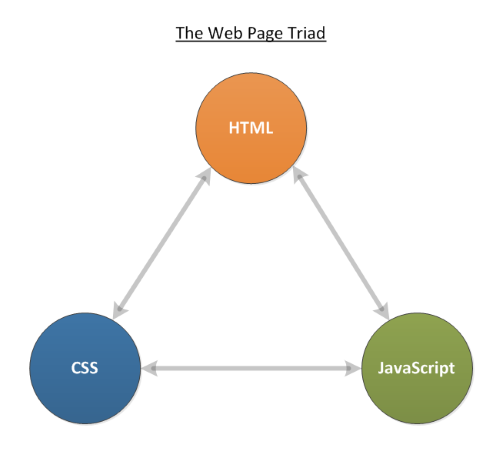
\includegraphics[width=0.6\linewidth]{triadJavaScript}
	\caption{Triade van de webpagina \autocite{itegrators2017}}
	\label{fig:Triade}
\end{figure}

Dankzij JavaScript is het mogelijk om de meeste elementen op een webpagina programmeerbaar te maken. Het wordt momenteel gebruikt op 95 procent van alle websites \autocite{W3Techs2019}. Het is ook de basis van andere scripttalen zoals TypeScript, waarvan Angular gebruik maakt.

Javascript wordt vaak verward met Java, maar dit is niet terecht. Ondanks dat beide talen enkele gelijkenissen vertonen, zijn er toch heel wat verschillen. De syntaxis van beide talen is gebaseerd op die van programmeertaal C. Samen met de naam van beide talen is dit de grootste gelijkenis. 

De verschillen zijn talrijk.
 Vooraleerst is Java een gecompileerde programmeertaal, terwijl JavaScript een geïnterpreteerde scripttaal is. Het verschil zit hem in de implementatie.  JavaScript kan direct geïnterpreteerd worden door de browser terwijl Java wordt gecompileerd naar bytecode aan de hand van een virtuele machine, namelijk de Java Virtual Machine (JVM). 

 Ten tweede is JavaScript loosely typed, dit wil zeggen dat we op voorhand niet moeten aangeven welke soort van informatie (boolean, string, int...) zal opgeslaan worden in een variabele. Dit zal pas gecontroleerd worden tijdens runtime. Java is strongly typed, hier moet het type steeds op voorhand gedeclareerd worden omdat de check reeds zal gebeuren bij compiletime. Dit maakt van JavaScript een meer flexibele taal maar helaas is JavaScript hierdoor ook gevoeliger voor bugs omdat de check pas later in het proces gebeurt.
 
 Een derde belangrijk verschil is dat van de concurrency. Java maakt gebruik van meerdere threads zodat het taken in parallel kan uitvoeren. JavaScript maakt gebruik van één main thread wat ervoor zorgt dat het in het algemeen trager werkt dan Java.
 
 Het laatste verschil is dat Java klasse gebaseerd is terwijl JavaScript prototype gebaseerd is. Bij klasse gebaseerde talen is er een top down hiërarchische structuur. 
 Een property  wordt gedefiniëerd in een klasse en zal overgeërfd worden door elke instantie van die klasse. Bij JavaScript is overerving prototypal, dit wil zeggen dat elk object kan erven van andere objecten.   
 
 \section{TypeScript}
 TypeScript is een open-source programmeertaal ontwikkeld door Microsoft. Het is een superset van JavaScript die ervoor zorgt dat statisch typen mogelijk wordt. Het werd in 2012 op de markt gebracht met de bedoeling om de ontwikkeling van grote applicaties eenvoudiger te maken. TypeScript wordt gecompileerd naar JavaScript wat ervoor zorgt dat gewone JavaScript applicaties ook geldige TypeScript applicaties zijn. 
 
 De voordelen van TypeScript ten opzichte van JavaScript zijn talrijk: het is een object-georiënteerde taal, compilation errors worden sneller gevonden door de TypeScript transpiler, het is een strongly-typed taal,... Bovendiendien is de populariteit van typescript enorm snel aan het stijgen. 
 
 De huidige versie van Typescript is TypeScript 3.4 en werd in maart 2019 uitgebracht.

\section{Framework}

Een software framework is een samenstelling van softwarecomponenten dat kan gebruikt worden bij het programmeren van applicaties. Het zal de tijd en kost voor het ontwikkelen van een applicatie aanzienlijk doen dalen. 
Het is een herbruikbaar raamwerk dat kan uitgebreid worden met zelf geschreven code. Software frameworks bestaan uit verschillende ondersteunende programma's, compilers, bibliotheken, tool sets en application programming interfaces (API).

Frameworks onderscheiden zich van gewone libraries aan de hand van drie kenmerken:

\begin{itemize}
	\item Inversion of control: Wanneer een methode uit een library wordt aangeroepen heeft de gebruiker de controle. Bij een framework is het het framework zelf dat de flow control bepaalt. 
	\item Uitbreidbaarheid: De gebruiker kan een framework uitbreiden of er gespecialiseerde code aan toevoegen om zo een specifieke functionaliteit toe te voegen. 
	\item Niet aanpasbare framework code: Hoewel de gebruiker het framework kan uitbreiden, mag hij de code niet aanpassen. Een framework volgt dus het open/closed-principe. 
	
\end{itemize}


\section{Component-gebaseerd Framework}
Een component-gebaseerd framework is een framework voor webapplicaties dat de verwerkingslogica opsplitst in verschillende onderdelen, genaamd componenten. 
Een component is dus een bouwsteen waaruit de applicatie is opgebouwd. Een component-gebaseerd framework bestaat uit veel verschillende componenten die variëren van heel klein tot heel groot zoals buttons, lijsten of volledige views. De component zorgt voor een eenvoudige configuratie van deze onderdelen. 


\section{Single Page Application}
Een Single Page Application (SPA) is een webapplicatie die draait op één enkele HTML webpagina. De HTML, CSS en JavaScript code wordt opgehaald in één laadactie van de pagina. De pagina zal daarna dynamisch bijgewerkt worden wanneer de gebruiker interageert met de webapplicatie (zie figuur \ref{fig:SPA}). Dankzij deze manier van werken is een Single Page Application vaak veel sneller dan een statische website, aangezien de statische website steeds opnieuw de inhoud moet laden. Alle JavaScript frameworks passen automatisch het Single Page Application concept toe. 

\begin{figure}[H]
	\centering
	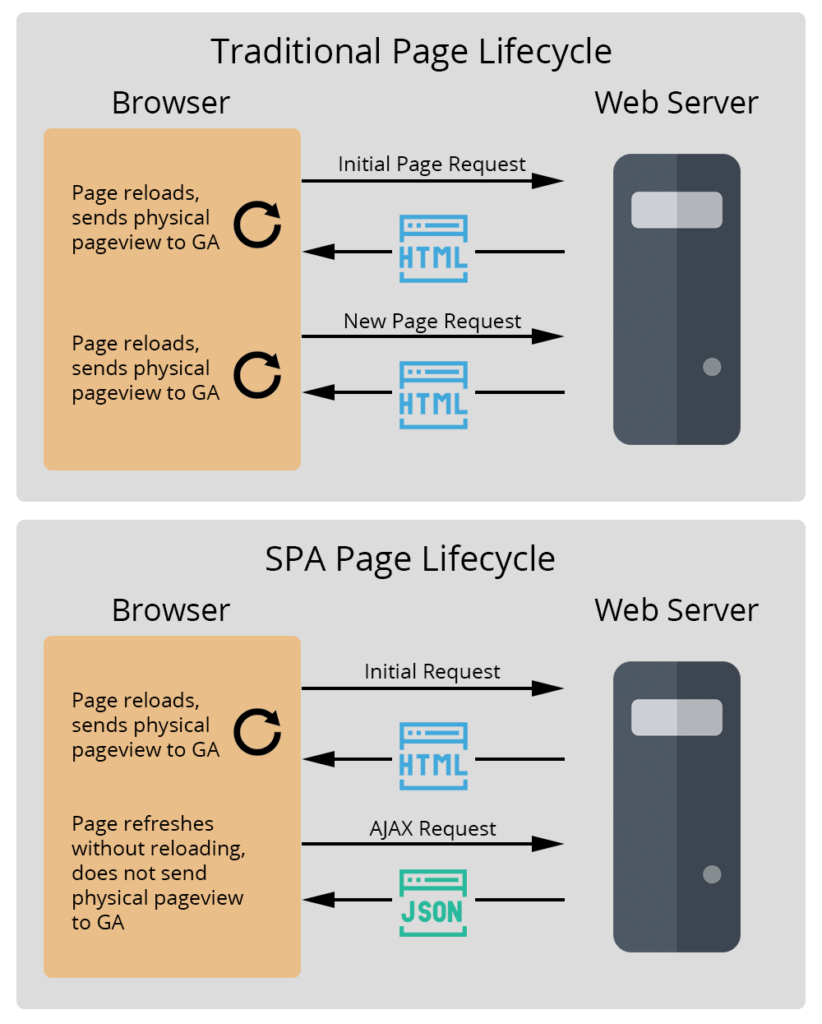
\includegraphics[width=0.5\linewidth]{spa-architecture}
	\caption{Statische website versus Single Page Application \autocite{E-nor2018}}
	\label{fig:SPA}
\end{figure}

\section{MVC}
De applicaties die opgebouwd zullen worden om beide frameworks te vergelijken zullen gebruik maken van het MVC(Model-View-Controller) patroon (zie figuur \ref{fig:Mvc} ). Daarom is het noodzakelijk om dit patroon kort te beschrijven.


Model View Controller is een ontwerppatroon dat een applicatie verdeelt in drie eenheden met verschillende verantwoordelijkheden:

	\textbf{Model}  \hspace{1cm} Het datamodel specifieert de logische structuur van de data in de applicatie. Het zal beschrijven hoe de data weergegeven wordt op niveau van de databank. Het datamodel beschrijft welke entiteiten verbonden zijn aan welke tabellen en hoe het zit met de relaties tussen deze datastructuren.   					\\ \\
	\textbf{View} \hspace{1cm} De view bepaalt hoe de data zal weergegeven worden op het scherm. Het doet geen verwerking van de gegevens maar wordt enkel gebruikt voor de interactie met de user. De userinterface-elementen worden allemaal gedefinieerd in dit onderdeel. 						\\	\\
	\textbf{Controller} \hspace{1cm} De controller verzorgt de interactie tussen de view en het model. De controller bestaat uit actions die reageren op de handelingen van de gebruiker. Aan de hand van die actions wordt het juiste model gebruikt en de passende view weergegeven.  			\\	\\
De voordelen van dit patroon zijn talrijk: de applicatie zal makkelijker uitbreidbaar worden, het ontwikkelingsproces zal sneller verlopen, dubbele code wordt vermeden, een model kan verschillende views toegewezen krijgen en modificatie van één van de drie eenheden zal geen invloed hebben op de andere eenheden.

\begin{figure}[H]
	\centering
	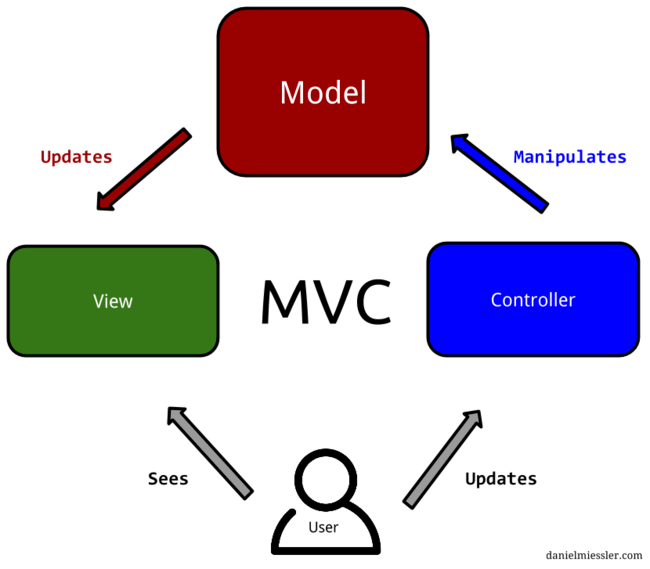
\includegraphics[width=0.6\linewidth]{MVC}
	\caption{Overzicht van het MVC patroon \autocite{DanielMissler2017}}
	\label{fig:Mvc}
\end{figure}

\section{Angular}
"Angular is a platform that makes it easy to build applications with the web. Angular combines declarative templates, dependency injection, end to end tooling, and integrated best practices to solve development challenges. Angular empowers developers to build applications that live on the web, mobile, or the desktop." \autocite{Angular2019} 

Angular is een front-end framework gebaseerd op TypeScript dat onderhouden wordt door het Angular Team van Google. Het is een volledig herschreven versie van AngularJS.
De belangrijkste bouwstenen van een Angular applicatie zijn de modules, componenten en services (zie figuur \ref{fig:Angular-Module-Component}).


\begin{figure}
\begin{lstlisting}[]
// imports
import { BrowserModule } from '@angular/platform-browser';
import { NgModule } from '@angular/core';
import { FormsModule } from '@angular/forms';
import { HttpClientModule } from '@angular/common/http';

import { AppComponent } from './app.component';
import { ItemDirective } from './item.directive';


// @NgModule decorator with its metadata
@NgModule({
declarations: [
AppComponent,
ItemDirective
],
imports: [
BrowserModule,
FormsModule,
HttpClientModule
],
providers: [],
bootstrap: [AppComponent]
})
export class AppModule { }
\end{lstlisting}
\caption{Angular root module voorbeeld}
\end{figure}


\subsection{Module}
Angular is een modulair framework, het is dus opgebouwd uit modules. Een module in Angular refereert naar een plaats waar componenten, directives, pipes en services gegroepeerd kunnen worden (zie figuur \ref{fig:Angular-Module-Component}). 
Het modulariteitssysteem van Angular heet NgModules en kan zowel functionaliteiten importeren die door andere NgModules worden geëxporteerd als zelf functionaliteiten exporteren. 
\\ \\
Elke Angular app heeft minstens één NgModule klasse, genaamd de root module. Gewoonlijk wordt deze de AppModule genoemd en wordt deze geplaatst in een file met de naam app.module.ts. Deze module zorgt voor het opstarten van de applicatie. 

\begin{figure}[H]
	\centering
	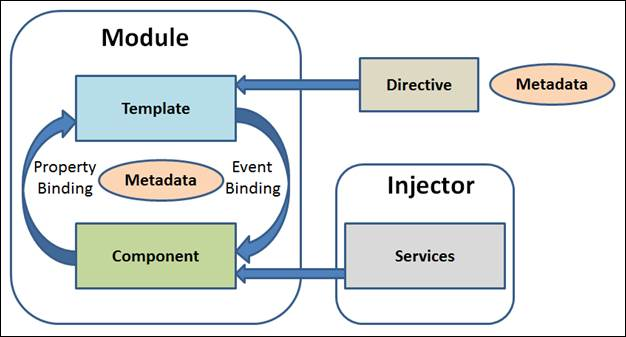
\includegraphics[width=0.6\linewidth]{Angular-Module-Component}
	\caption{Overzicht van de Angular bouwstenen \autocite{Trivedi2016}}
	\label{fig:Angular-Module-Component}
\end{figure}

\textbf{NgModule metadata} \hspace{1cm} Een NgModule wordt steeds gedefinieerd door een klasse met de decorator @NgModule(). Deze decorator is een functie dat een metadata object gebruikt om de module te beschrijven. De belangrijkste attributen van dit object zijn de volgende: 
\begin{itemize}
	\item declarations: De componenten, directives en pipes die toebehoren aan deze module.  
	\item exports: De subset van declaraties dat andere NgModules moeten kunnen importeren. 
	\item imports: Andere modules die nodig zijn binnen deze NgModule. 
	\item providers: Services die deze NgModule gebruikt. Providers die op dit niveau worden gedeclareerd kunnen over de hele app gebruikt worden. Het is echter ook mogelijk om providers te declareren op niveau van componenten, wat vaak een betere optie is.
	\item bootstrap: Dit attribuut moet enkel ingesteld worden door de root NgModule. Het bepaalt de algemene view die alle andere views beheert.
\end{itemize}

Het NgModule systeem is verschillend van het JavaScript module systeem voor het beheren van collecties van JavaScript objecten. Het NgModule systeem en het JavaScript module systeem zijn complementaire systemen die kunnen gecombineerd worden bij het schrijven van applicaties. 

\subsection{Component}
Componenten zijn de eenvoudigste bouwstenen van een angular applicatie. Ze beheren een deel van het scherm dat bekend staat als een view. Binnen een MVC context zouden ze omschreven worden als een controller. Een component behoort steeds toe aan een NgModule, zodanig dat het beschikbaar kan zijn voor een andere component of applicatie. 

Een component heeft verschillende lifecycle hooks (zie figuur \ref{fig:lifecyclehooks}), zoals de ngOnInit(). In elk van deze lifecycle hooks kan je applicatie bepaalde acties uitvoeren. Angular zal componenten automatisch aanmaken, updaten en verwijderen terwijl de gebruiker navigeert door de applicatie. 

\begin{figure}[H]
	\centering
	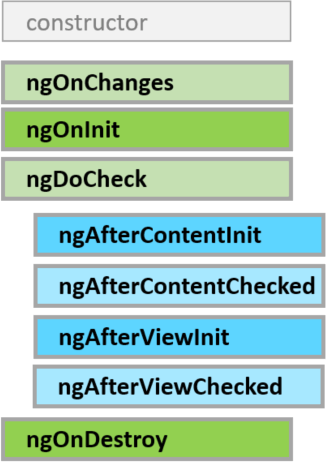
\includegraphics[width=0.6\linewidth]{lifecyclehooks}
	\caption{De lifecycle hooks \autocite{dartlang2019}}
	\label{fig:lifecyclehooks}
\end{figure}

\textbf{Component metadata} \hspace{1cm} Een component klasse is een klasse die wordt geïdentificeerd aan de hand van de @Component decorator. Deze klasse zal de metadata van de component bevatten. De metadata van een component laat aan Angular weten waar ze de bouwstenen kan vinden die nodig zijn om de component en zijn view aan te maken. De combinatie van een component met zijn template zorgen voor een view. 
De belangrijkste configuratieopties van een component zijn de volgende:
\begin{itemize}
	\item selector: De selector vertelt Angular om een component te maken op de plaats waar het de corresponderende tag vindt in de HTML. 
	\item templateUrl: Het adres van de HTML template die gelinkt is aan de component. Dit adres is relatief aan de module. 
	\item providers: Services die door deze component gebruikt worden. Deze worden weergegeven in een array. 
\end{itemize}

\textbf{Template en views} \hspace{1cm} De view van een component wordt steeds gedefiniëerd aan de hand van een bijhorende template. De template is een HTML form dat Angular de informatie doorgeeft die nodig is om de component weer te geven. Views worden hiërarchisch geordend, waardoor het mogelijk is om volledige onderdelen van de user interface aan te passen of te verbergen. De template die rechtstreeks geassocieerd is met de component noemt men de host view. Deze host view kan embedded views bevatten die beheerd worden door andere componenten. Deze componenten kunnen zich in een andere NgModule bevinden. 

\textbf{Data binding} \hspace{1cm} Databinding is het proces dat zorgt voor een connectie tussen de interface van de applicatie en het model. Wanneer de data verandert van waarde, zal de interface ook aangepast worden. Het opstellen van zo een mechanisme is een moeilijke en arbeidsintensieve taak. Gelukkig is dit met Angular eenvoudig te implementeren. Angular voorziet zelfs in two-way binding, wat inhoudt dat ook het model kan aangepast worden via de interface, bijvoorbeeld door het invullen van een formulier. Angular voorziet in drie verschillende manieren om data te binden:
\begin{itemize}
	\item interpolation: Techniek om waardes te binden aan een User Interface element.
	Deze techniek kan enkel gebruikt worden bij one-way binding van component naar view. Interpolation gebruikt als scheidingsteken de dubbele accolades \{\{ en \}\}. Interpolation is een speciale syntax die door Angular wordt geconverteerd naar property binding.
	\item property binding: Techniek om waardes te binden aan DOM attributen van de HTML elementen. Zo kunnen de attributen van view elementen ingesteld worden, zoals de bron van een afbeelding. Net zoals interpolation kan deze techniek enkel gebruikt worden bij one-way binding van component naar view. De scheidingstekens van property binding zijn de vierkante haakjes [ en ].
	\item event binding: Wanneer users interageren met de applicatie zoals een click of een actie van het toetsenbord kan dit via event binding opgevangen worden. Event binding is een one-way binding maar in tegenstelling tot de voorgaande technieken werkt deze van view naar component. De scheidingstekens van event binding zijn de ronde haakjes ( en ). 
\end{itemize}
Door bovenstaande one-way binding technieken te combineren is het in Angular mogelijk om two-way binding te bekomen. 

\textbf{pipes} \hspace{1cm} Dankzij pipes is het mogelijk om waardes die worden weergegeven in de template HTML te transformeren. Een klasse met de @Pipe decorator definieert een functie die input waardes transformeert naar output waardes voor een view. Angular voorziet al enkele pipes zoals de date pipe of de currency pipe, maar het is ook mogelijk om zelf pipes te maken. Om een transformatie in een HTML template te specifiëren gebruikt men de pipe operator: |. 

\textbf{directives} \hspace{1cm} De templates van Angular zijn dynamisch. Wanneer ze weergegeven worden zullen ze getransformeerd worden volgens de instructies die meegegeven worden door directives. Een directive is een klasse met de @Directive() decorator. Er zijn twee soorten directives: structural en attribute. 

De structural directives kunnen elementen verwijderen, toevoegen of vervangen in de DOM. Er zijn twee automatisch ingebouwde structural directives: de NgFor die iteraties uitvoert en de nfIf die een check uitvoert op condities.

De attribute directives kunnen het gedrag of het voorkomen van een bestaand element aanpassen. In de templates lijken ze op gewone HTML attributen, vandaar ook de naam. 
Een voorbeeld van een attribute directive is de ngModel die zorgt voor two-way data binding. Het verandert het gedrag van een bestaand element zoals bijvoorbeeld <input>. 

\subsection{Service}
Service is een brede naam voor elke waarde, functie of feature dat een applicatie nodig heeft. Een service is een klasse met een zeer specifiek doel. Het grote verschil tussen een component en een service is het feit dat een component gelinkt is aan een view, terwijl een service dat niet is. \\
Een component kan bepaalde taken delegeren aan een service, zoals het ophalen van data van een server of het valideren van de input van een gebruiker. De services kunnen hergebruikt worden over de hele applicatie waardoor er minder redundante code zal ontstaan. Bovendien zorgen ze er ook voor dat componenten niet te groot worden. 

\textbf{dependency injection} \hspace{1cm} services worden geïnjecteerd in een component, waardoor deze components toegang hebben tot die service klasse.De service klasse heeft geen specifieke decorator, maar maakt gebruik van de @Injectable() decorator. Deze zorgt ervoor dat Angular de klasse kan injecteren in een component als een dependency. Een dependency hoeft geen service te zijn, maar kan evenwel een functie of een waarde zijn. 

Wanneer Angular ontdekt dat een component een dependency heeft op een service, zal het eerst nakijken of er al bestaande instanties zijn van die service. Als die er nog niet zijn, dan zal de injector er een aanmaken, gebruik makend van de provider van de service. Pas wanneer alle services aangemaakt zijn kan Angular de constructor van de component aanroepen, met de services als argumenten. 

Elke service moet minstens één provider hebben. Deze kan deel uitmaken van de metadata van de service, of kan geregistreerd worden in specifieke modules of componenten. 

\section{Vaadin}
Vaadin is een platform voor de ontwikkeling van webapplicaties. Het Vaadin platform bestaat uit enkele verschillende onderdelen zoals web components, een reeks tools en een Java web framework genaamd Vaadin Flow. Wanneer in deze paper gesproken wordt over Vaadin, hebben we het eigenlijk over het framework Vaadin Flow, wat het belangrijkste onderdeel is van het Vaadin platform. 
\subsection{Vaadin Flow}

"Vaadin Flow connects the Java ecosystem to your web platform. Flow is an integral part of the Vaadin platform." \autocite{Vaadin2019} 

Vaadin Flow is een framework om moderne web apps en websites te bouwen. Het zorgt ervoor dat Java gebruikers gebruik kunnen maken van web componenten. Dankzij Vaadin Flow kunnen op een zeer snelle wijze user interfaces gemaakt worden in Java en kunnen deze eenvoudig gekoppeld worden aan iedere Java backend.

De grootste voordelen van Vaadin Flow zijn de volgende:
\begin{itemize}
	\item Een reeks voorgedefinieerde user interface componenten.
	\item abstractielagen die ervoor zorgen dat zelfgemaakte componenten eenvoudig hergebruikt kunnen worden.
	\item Two-Way Data binding API
	\item Router API
\end{itemize}

\subsection{Component}
Het Vaadin platform heeft een reeks van componenten met server-side Java API's die gebruikt kunnen worden om een webapplicatie op te bouwen. Deze componenten zitten verwerkt als dependencies in het platform. Via de vaadin-core module krijgt men direct toegang tot alle open source componenten zoals Textfield, Button en Grid. De vaadin module breidt dit nog uit met alle officieel ondersteunde componenten in het Vaadin platform zoals bijvoorbeeld Vaadin Charts. 

\textbf{Data binding} \hspace{1cm} Vaadin heeft een klasse die gespecialiseerd is in het binden van data, genaamd de Binder klasse. Aan de hand van deze klasse kan de ontwikkelaar bepalen welke waardes gebonden worden aan bepaalde invoervelden in de user interface. De Binder klasse zal de gegevens die de gebruiker invoert lezen en converteren naar het type dat verwacht wordt in het model. De Binder klasse kan enkel gebruikt worden op componenten die een HasValue property hebben, zoals een Textfield of een ComboBox. 

\textbf{Data validatie} \hspace{1cm} De Binder klasse kan meer dan enkel data binden: het kan ook de validatie van de user input doen. Hiervoor moet er een Validator aangemaakt worden. Deze validators zullen de input valideren op twee momenten: 
\begin{itemize}
	\item Telkens wanneer de gebruiker de waardes in het veld verandert.
	\item Wanneer de data wordt weggeschreven naar de bean. 
\end{itemize}

\textbf{Data conversie} \hspace{1cm} De Binder klasse kan ook de waarde types uit de user input converteren naar de waarde types van het model. Dit kan handig zijn in heel veel situaties, zoals wanneer de users enkel cijfers mogen invullen in een invoerveld.
Om deze data conversie te bekomen moet men een Converter aanmaken. Deze Converter wordt dan gekoppeld aan een Binder. Aan een Binder object kunnen meerdere converters gekoppeld worden. 

\subsection{Routing}
Routing gebeurt in Vaadin aan de hand van de Router klasse. De router zorgt ervoor dat de juiste content wordt weergegeven wanneer een gebruiker navigeert binnen de applicatie. Elke component kan als route ingesteld worden via de @Route annotatie. 
Het pad naar deze component kan als argument meegegeven worden aan de annotatie, bijvoorbeeld: @Route("docs/hello").

\textbf{Navigatie Lifecycle} \hspace{1cm} De navigatie lifecycle bestaat uit een aantal evenementen die gebeuren wanneer een user navigeert van één view naar een andere. Deze zullen hieronder kort besproken worden in volgorde waarin ze voorkomen. 

\begin{itemize}
	\item BeforeLeaveEvent: Deze lifecycle kan de navigatie uitstellen, annuleren of veranderen naar een andere bestemming. Dit kan bijvoorbeeld handig zijn wanneer er aan de gebruiker gevraagd moet worden of ze hun niet-opgeslagen veranderingen willen opslaan voordat ze navigeren naar een andere view. 
	\item BeforeEnterEvent: Dit evenement kan de navigatie veranderen naar een bestemming die verschilt van de originele. Op deze wijze kan men reageren op speciale situaties, zoals wanneer er geen data is om weer te geven of wanneer de gebruiker niet over de gepaste permissies beschikt.
	\item AfterNavigationEvent: In dit evenement worden delen van de user interface geüpdatet nadat de navigatie volbracht is. Dit kan gebruikt worden om het menu item dat actief is te markeren in een andere kleur.
\end{itemize}

\textbf{RouterLink component} \hspace{1cm} De RouterLink component kan content van een nieuwe component ophalen zonder de pagina te herladen. De pagina wordt geüpdatet wat veel sneller gaat dan een nieuwe pagina te laden. 


%%=============================================================================
%% Methodologie
%%=============================================================================

\chapter{Methodologie}
\label{ch:methodologie}

%% TODO: Hoe ben je te werk gegaan? Verdeel je onderzoek in grote fasen, en
%% licht in elke fase toe welke stappen je gevolgd hebt. Verantwoord waarom je
%% op deze manier te werk gegaan bent. Je moet kunnen aantonen dat je de best
%% mogelijke manier toegepast hebt om een antwoord te vinden op de
%% onderzoeksvraag.

\section{Requirements-analyse}
Om een goede analyse te maken van beide frameworks moeten er requirements opgesteld worden. Aan de hand van deze requirements zullen de frameworks beoordeeld worden. De requirements bestaan uit functionele en niet-functionele requirements. Beide frameworks zullen een score toegewezen krijgen voor elk van de requirements. De scores gaan van 1(zwak) tot 5(uitstekend).

\begin{itemize}
\item  Functionele requirements 
\begin{itemize}
	\item Ondersteuning voor mobile
	\item Compatibiliteit met verschillende browsers
	\item Uitgebreide mogelijkheden rond testing
	\item Beschikbare voorgedefiniëerde componenten 
	\item Ondersteuning voor data binding
	\item Goede performantie
\end{itemize}

\item Niet-functionele requirements
\begin{itemize}
	\item Moet over een goede documentatie beschikken
	\item Moet over een grote community beschikken
	\item Moet relatief makkelijk aan te leren zijn 
	\item Moet open source zijn	
\end{itemize}
\end{itemize}

Deze functionele en niet-functionele requirements zullen nu ingedeeld worden volgens de MoSCoW methode.\autocite{ProductPlan2019}
De 'Must-have initiatives' zijn noodzakelijk voor het framework en moeten dus aanwezig zijn.
De 'Should-have initiatives' zijn een stapje lager dan de must-haves. Ze zijn belangrijk voor het framework maar niet noodzakelijk.
Ten slotte zijn er nog de 'Could-have initiatives'. Deze mogen omschreven worden als nice-to-have. Het is positief indien een framework hieraan voldoet, maar het is geen noodzakelijkheid.

\begin{itemize}
	\item  Must-have initiatives
	\begin{itemize}
	\item Ondersteuning voor mobile
	\item Compatibiliteit met verschillende browsers
	\item Ondersteuning voor data binding
	\item Moet relatief makkelijk aan te leren zijn
	\item Moet open source zijn	 
	\end{itemize}
	\item Should-have initiatives
	\begin{itemize}
	\item Uitgebreide mogelijkheden rond testing
	\item Beschikbare voorgedefiniëerde componenten 
	\item Goede performantie
	\item Moet over een goede documentatie beschikken
	\end{itemize}
		\item Could-have initiatives
		\begin{itemize}
	\item Moet een populair framework zijn met een grote community
		\end{itemize}
\end{itemize}

Om meer inzicht te krijgen in de materie werd een gelijkaardige contactapplicatie gebouwd in zowel Angular (Zie figuur \ref{fig:ContactapplicatieAngular} ) als Vaadin (Zie figuur \ref{fig:ContactapplicatieVaadin} ). In voorgenoemde applicatie kunnen via een formulier nieuwe contacten toegevoegd worden. Beide applicaties werden verbonden met een Spring Boot backend. Deze programma's zijn beschikbaar op volgende locaties:
\begin{itemize}
	\item Frontend Angular: \url{https://github.com/Beazar/BPAngular}
	\item Spring Boot backend voor Angular: \url{https://github.com/Beazar/BPBackend}
	\item Full stack Vaadin: \url{https://github.com/Beazar/BPVaadin}
\end{itemize}

\begin{figure}[H]
	\centering
	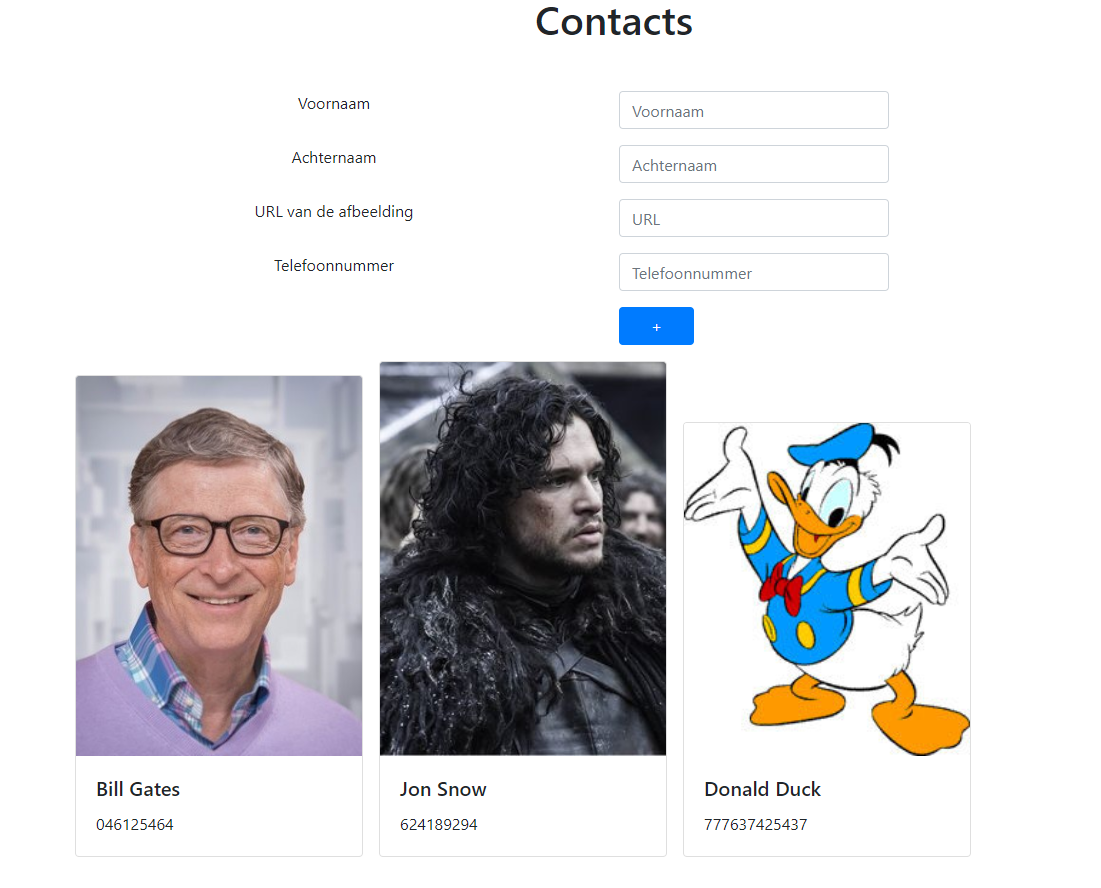
\includegraphics[width=0.6\linewidth]{AngularApp}
	\caption{Contactapplicatie Angular}
	\label{fig:ContactapplicatieAngular}
\end{figure}

\begin{figure}[H]
	\centering
	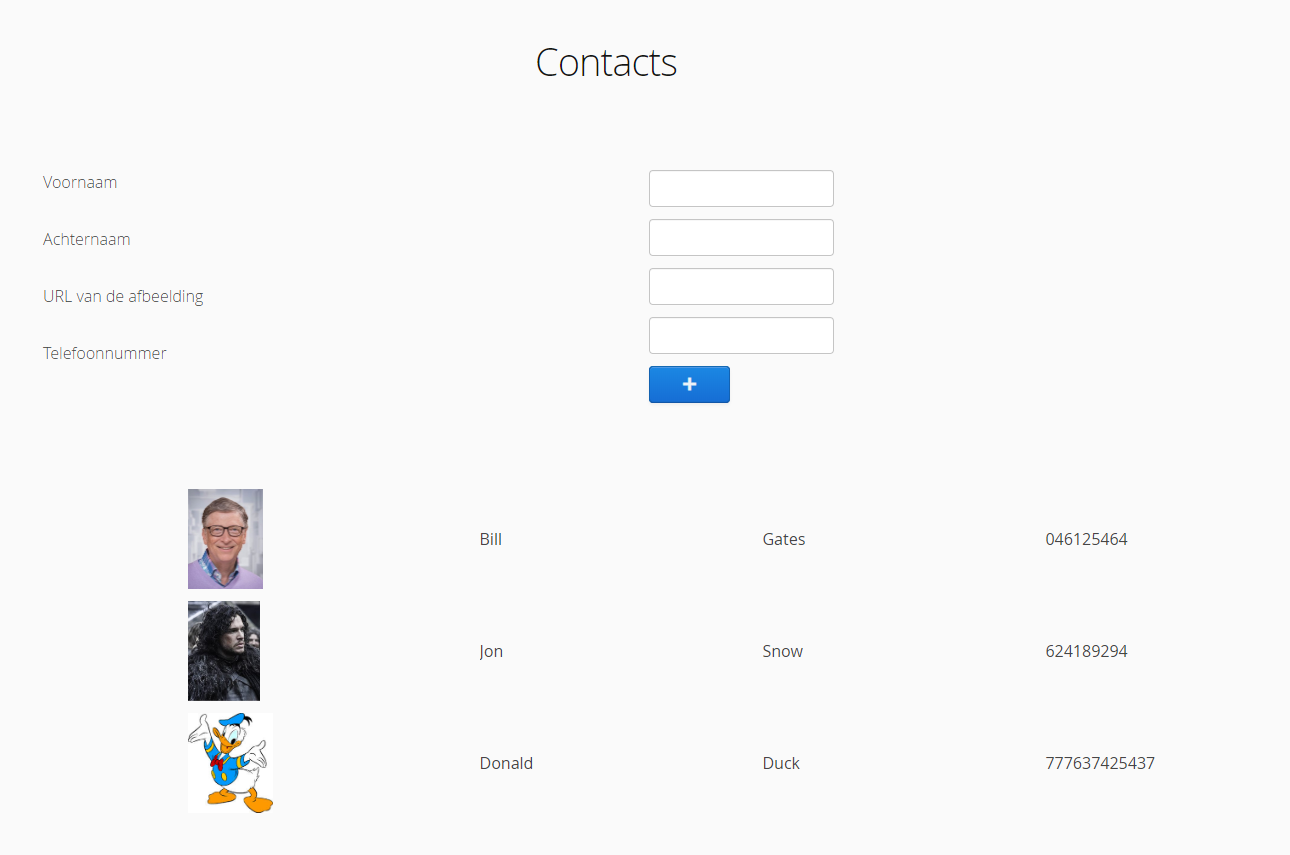
\includegraphics[width=0.6\linewidth]{VaadinApp}
	\caption{Contactapplicatie Vaadin}
	\label{fig:ContactapplicatieVaadin}
\end{figure}


\input{angular}
\input{vaadin}

% Voeg hier je eigen hoofdstukken toe die de ``corpus'' van je bachelorproef
% vormen. De structuur en titels hangen af van je eigen onderzoek. Je kan bv.
% elke fase in je onderzoek in een apart hoofdstuk bespreken.

%\input{...}
%\input{...}
%...

%%=============================================================================
%% Conclusie
%%=============================================================================

\chapter{Conclusie}
\label{ch:conclusie}

%% TODO: Trek een duidelijke conclusie, in de vorm van een antwoord op de
%% onderzoeksvra(a)g(en). Wat was jouw bijdrage aan het onderzoeksdomein en
%% hoe biedt dit meerwaarde aan het vakgebied/doelgroep? Reflecteer kritisch
%% over het resultaat. Had je deze uitkomst verwacht? Zijn er zaken die nog
%% niet duidelijk zijn? Heeft het onderzoek geleid tot nieuwe vragen die
%% uitnodigen tot verder onderzoek?




%%=============================================================================
%% Bijlagen
%%=============================================================================

\appendix

%%---------- Onderzoeksvoorstel -----------------------------------------------

\chapter{Onderzoeksvoorstel}

Het onderwerp van deze bachelorproef is gebaseerd op een onderzoeksvoorstel dat vooraf werd beoordeeld door de promotor. Dat voorstel is opgenomen in deze bijlage.

% Verwijzing naar het bestand met de inhoud van het onderzoeksvoorstel
%---------- Inleiding ---------------------------------------------------------

\section{Introductie} % The \section*{} command stops section numbering
De keuze uit de bestaande frameworks wordt steeds moeilijker door het groeiende aantal opties. Deze bachelorproef zal een antwoord formuleren op de volgende onderzoeksvraag: in welke situatie kiest men best voor het Vaadin framework en wanneer opteert men best voor Angular? Dit onderzoek zal de keuze tussen twee populaire component based frameworks, Vaadin en Angular, vereenvoudigen. Uit onderzoek van ~\textcite{Schlosser2018} blijkt dat Angular op de tweede plaats komt qua populariteit terwijl Vaadin de achtste plaats bezet. 

%---------- Stand van zaken ---------------------------------------------------

\section{State-of-the-art}
\label{sec:state-of-the-art}

Het belangrijkste verschil tussen de twee frameworks is de programmeertaal waarmee de frameworks werken. Vaadin werkt voornamelijk met Java maar kan ook werken met andere JVM talen zoals Javascript. Angular werkt met HTML, CSS en Typescript of Javascript.  Een tweede belangrijk verschil is dat Angular een frontend framework is in tegenstelling tot Vaadin dat zowel frontend als backend in zijn framework omvat.
Een derde verschil is dat Angular gebruik maakt van een Mobile-first aanpak, wat niet het geval is bij Vaadin.
Ten slotte is Angular beter geschikt voor applicaties die schaalbaar moeten zijn voor een groot aantal gebruikers. Vaadin krijgt moeilijkheden wanneer er meer dan 100.000 gelijktijdige gebruikers zijn. 

In 2017 is er een vergelijkbaar onderzoek uitgevoerd door \textcite{Hellberg2017} waaruit blijkt dat de keuze tussen Vaadin en Angular afhankelijk is van een aantal factoren zoals: kwaliteiten van het team, de verwachtingen omtrent schaalbaarheid en onderhoud, beveiliging en de eisen voor mobile.
In het onderzoek van Hellberg werd gewerkt met Vaadin 8 en Angular 4.

Dit onderzoek zal zich onderscheiden van bovenstaand onderzoek door te werken met nieuwe releases, namelijk Vaadin 10 en Angular 7. 

% Voor literatuurverwijzingen zijn er twee belangrijke commando's:
% \autocite{KEY} => (Auteur, jaartal) Gebruik dit als de naam van de auteur
%   geen onderdeel is van de zin.
% \textcite{KEY} => Auteur (jaartal)  Gebruik dit als de auteursnaam wel een
%   functie heeft in de zin (bv. ``Uit onderzoek door Doll & Hill (1954) bleek
%   ...'')


%---------- Methodologie ------------------------------------------------------
\section{Methodologie}
\label{sec:methodologie}

De frameworks zullen vergelijkingen ondergaan op verschillende vlakken zoals de architectuur en structuur van het framework, populariteit,  het werken met data, mobile ondersteuning, testing, onderhoud en performantie. Deze vergelijking zal gebeuren aan de hand van een simulatie waarbij een applicatie tweemaal wordt opgebouwd. De eerste keer gebeurt dit aan de hand van het Vaadin framework, de tweede keer aan de hand van Angular. 
%---------- Verwachte resultaten ----------------------------------------------
\section{Verwachte resultaten}
\label{sec:verwachte_resultaten}

De verwachte resultaten houden in dat het opzetten van een webapplicatie aan de hand van Vaadin eenvoudiger zal zijn dan aan de hand van Angular. Het aanpassen van de applicatie zal echter eenvoudiger zijn in Angular omdat hier gewerkt wordt met CSS. Dit houdt in dat ook ontwerpers die niet geschoold zijn in het programmeren kunnen meewerken aan de look-and-feel van de applicatie. 
Qua mobile support kan er verwacht worden dat Angular beter zal scoren dan Vaadin, dankzij zijn mobile-first approach.
De performantie van Vaadin zou hoger moeten liggen dan die van Angular in de eerste keer dat de applicatie geladen wordt. De volgende keren zouden de laadtijden gelijkaardig moeten zijn. 
Ten slotte zal Vaadin beter scoren op vlak van beveiliging omdat Angular gebruik maakt van third party UI components, wat de ondersteuning fragiel maakt. 

%---------- Verwachte conclusies ----------------------------------------------
\section{Verwachte conclusies}
\label{sec:verwachte_conclusies}

Naar verwachting zullen beide frameworks hun toepassingen kennen in verschillende situaties. Geen van beide frameworks zal beduidend beter zijn dan het andere, maar in verschillende situaties zal er geopteerd worden voor verschillende frameworks. Voor het starten van een project moet eerst een duidelijke analyse gemaakt worden van de requirements om zo te bepalen welk framework de beste resultaten zal bieden. Parameters zoals daar zijn beveiliging, kwaliteiten van het team en schaalbaarheid zullen een belangrijk onderdeel zijn van de uiteindelijke beslissing. Bovendien zal de scholing van de programmeur vaak doorslaggevend zijn in de eindbeslissing. Een Java programmeur zal zich hoogstwaarschijnlijk comfortabeler voelen met het Vaadin framework, terwijl een Typescript programmeur sneller zal kiezen voor het Angular framework. 



%%---------- Andere bijlagen --------------------------------------------------
% TODO: Voeg hier eventuele andere bijlagen toe
%\input{...}

%%---------- Referentielijst --------------------------------------------------

\printbibliography[heading=bibintoc]
%\addcontentsline{toc}{chapter}{\textcolor{maincolor}{\IfLanguageName{dutch}{Bibliografie}{Bibliography}}}

\end{document}
